\documentclass[twocolumn,a4wide,parskip,10pt]{scrartcl}

\usepackage[english]{babel}
\usepackage[utf8]{inputenc}

\usepackage{a4wide}

\usepackage[pdftex,
  pdfauthor={Michael Schupikov},
  pdftitle={System description for cress.space},
  pdfsubject={System description for cress.space},
  pdfkeywords={system description, cress.space},
  pdfproducer={Latex},
  pdfcreator={pdflatex}]{hyperref}

\title{System setup cress.space}
\date{\today}
\author{Team cress.space}

\usepackage{lmodern}
\renewcommand*\familydefault{\sfdefault}

\usepackage[automark,headsepline]{scrlayer-scrpage}

\usepackage{lastpage}
\clearpairofpagestyles
\lohead{\textsc{System setup}}
\lehead{\textsc{System setup}}
\rohead{\textsc{cress.space}}
\rehead{\textsc{cress.space}}
\cfoot{\thepage \hspace{1pt} / \pageref{LastPage}}
\lofoot{\footnotesize v1.0}
\rofoot{\footnotesize \today}
\pagestyle{scrheadings}

\usepackage{graphicx}
\graphicspath{ {data/} }

\begin{document}

% Titlepage
\maketitle
%\clearpage
\setcounter{page}{1}

\section{Setup}

The environment for the cress is controlled by various factors that
can be manipulated by actors. The information about the current state
of the environment is collected by sensors. All those actors and
sensors are managed by a Raspberry Pi device which is controlled by an
API accessible from the web. See figure \ref{fig:overview_api_raspi}
for illustration.

The actors and sensors are as follows.

\begin{tabular}{p{2.5cm}p{4cm}}
  433MHz Transmitter & \\
  DHT 22 & Get Temperature and humidity.\\
  White LEDs & Light for elumination at night.\\
  Pump 1 & Pump to transfer water to the cress.\\
  Pump 2 & Pump to transfer water back to the water supply tank.\\
  Pelier Elements & Change temperature of the environment.\\
  Water Level & Get water level.
\end{tabular}

The corresponding webpage is \url{https://cress.space/}. Information about
the environment is provided here. By voting, users can decide which
actions should be taken to modify the environment in which the cress
is growing.

\begin{figure*}[!h]
  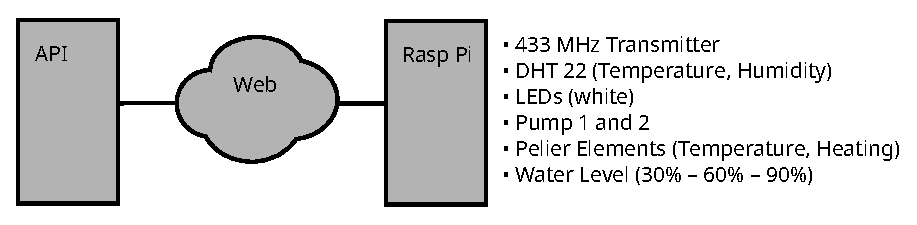
\includegraphics{overview_api_raspi.eps}
  \label{fig:overview_api_raspi}
  \caption{Setup for cress.space}
\end{figure*}

\paragraph{Push-Request.}

Every 10 minutes the UV light is turned off while the LEDs are turned
on. Then a picture is taken, which gets pushed to the API together
with collected sensor data.

\paragraph{Pull-Request.}

The parameters are determined by voting on the webpage. Then they
are sent to the Raspberry Pi device, which in turn applies them to the
available actors to manipulate the environment for the cress.

\appendix

\section{Scripts}

In \path{functions.sh} all the necessary shell functions are
defined. The functions are

\begin{tabular}{ll}
  \texttt{SwitchPumpOn} & Turn on the water pump.\\
  \texttt{SwitchPumpOff} & Turn off the water pump.\\
  \texttt{SwitchUVOn} & Turn on the UV light.\\
  \texttt{SwitchUVOff} & Turn off the UV light.\\
  \texttt{SwitchLEDOn} & Turn on the white LED light.\\
  \texttt{SwitchLEDOff} & Turn off the white LED light.\\
  \texttt{PushSensorData} & Send data to API.
\end{tabular}

The script \path{oneshot.sh} is called periodically via
\texttt{crontab} and implements one single data transfer cycle between
API and Raspberry Pi.

\end{document}

